\documentclass[pdflatex,sn-basic]{sn-jnl}

\usepackage{graphicx}
\usepackage{booktabs}
\usepackage{multirow}
\usepackage{amsmath,amssymb}
\usepackage{textcomp}
\usepackage{xcolor}
\usepackage{tabularx}
\usepackage{array}
\let\orcidlogo\relax
\usepackage{orcidlink}

\newcolumntype{Y}{>{\raggedright\arraybackslash}X}
\newcommand{\ha}{\,ha}
\newcommand{\kmsq}{\,km$^{2}$}

\raggedbottom

\begin{document}

\articletype{Methodology Article}

\title[Use-conditioned due diligence for GeoAI products]{A use-conditioned due-diligence protocol for open AI-derived geospatial products: Application to Fields of The World in Türkiye}

\author*[1,2]{\fnm{Yunus Serhat} \sur{B\i{}\c{c}ak\c{c}\i{}}\orcidlink{0000-0002-7288-9959}}
\email{yunus.serhat@marmara.edu.tr}

\affil[1]{\orgdiv{Department of Artificial Intelligence and Machine Learning},
\orgdiv{Faculty of Applied Sciences},
\orgname{Marmara University},
\orgaddress{\city{Istanbul}, \country{Türkiye}}}

\affil[2]{\orgdiv{Geospatial Data Science Group},
\orgdiv{School of Geographical \& Earth Sciences},
\orgname{University of Glasgow},
\orgaddress{\city{Glasgow}, \country{United Kingdom}}}

\abstract{Users of open geospatial products derived by machine learning must often make an adoption decision before independent reference data are available. This article presents a use-conditioned, decision-oriented due-diligence protocol that begins with intended use, decision risk and target ontology; tests product identity, population, geometry, topology, threshold sensitivity, attribute semantics, denominator provenance, cross-layer consistency and reproducibility; and returns adopt, adopt with restrictions, external validation required or reject for the declared use. The protocol operationalises, but does not replace, geographic data quality, provenance and documentation frameworks. It is demonstrated on the Fields of The World (FTW) layers over Türkiye, for which no country-specific reference evaluation is reported. With no analyst-imposed area floor, the reconciled 2024 and 2025 layers contain 14,139,788 and 15,075,042 mapped units, with summed polygon areas of 21.08 and 21.53 million ha. Exact tiled unions find only 0.074 ha of repeated footprint in 2024 and none beyond numerical tolerance in 2025, whereas units at least 100 ha contribute 28.11\% and 29.00\% of the summed areas. A documented 400 m$^{2}$ scenario removes 21.45\% and 24.22\% of units and raises medians by 67.74\% and 85.08\%. Null confidence means no sampled value, making national filtering inappropriate. Province aggregates correspond closely across layers, but offsets cannot be attributed uniquely to product behaviour or landscape change. The case supports restricted exploration and sampling design, requires local validation for quantitative monitoring, and rejects cadastral, registry and eligibility uses.}

\keywords{geospatial data quality, provenance, reproducibility, open data products, GeoAI}

\maketitle

\section{Introduction}\label{sec:introduction}

Open geospatial products derived by machine learning are now published faster than the community can independently assess them, and availability is not evidence of fitness for a particular use. The informatics problem is not merely whether a file can be opened. A user must connect machine-readable geometry and metadata to a target phenomenon, a decision context, explicit tolerances and an auditable action. The Fields of The World (FTW) programme illustrates this problem. It comprises a machine-learning benchmark, a segmentation workflow, practitioner guidance and a distributed global prediction product \citep{corley_fields_2026,muhawenayo_prue_2026,robinson_first_2026}, released through Source Cooperative as nominal annual national partitions under an open licence \citep{fields_of_the_world_global_2026}. A ready-made layer lowers the technical barrier to adoption, but users still need to establish what the polygons represent, how attributes were derived, whether administrative joins are complete, how filtering choices affect summary statistics and whether different product layers agree in both ranking and level.

Products of this kind sit at the end of a long methodological lineage. Field boundaries provide spatial units for crop mapping, yield assessment and land management. Remote sensing and geographic information systems have long supported resource inventories in Türkiye, including the development of greenhouse databases that revealed differences between remotely derived and administrative area estimates \citep{sonmez_use_2006}. More recent research has applied remote sensing driven by artificial intelligence to regional crop-growth monitoring and production forecasting \citep{wang_analysis_2026}. Automatic delineation has progressed from Landsat time series \citep{white_contemporary_2015,yan_conterminous_2016} to deep learning applied to Sentinel-2 imagery \citep{persello_delineation_2019,diakogiannis_resunet-_2020,waldner_deep_2020,waldner_detect_2021}. More broadly, hybrid convolutional and transformer architectures have been used for geospatial object segmentation \citep{bicakci_attransunet_2023}. Open benchmarks have made methods more comparable and reusable \citep{dandrimont_ai4boundaries_2023,kerner_fields_2025}, and recent work extends the progression to global field-boundary products at 10 m resolution \citep{corley_fields_2026,muhawenayo_prue_2026,robinson_first_2026}.

The gap between what a product represents and what a user assumes it represents is especially consequential in Türkiye, where agricultural holdings commonly comprise several land parcels and fragmentation remains a central land-management concern \citep{sklenicka_classification_2016,turkish_statistical_institute_agricultural_2018,tanrivermis_assessment_2024}. Consolidation and diversification studies show that this remains an active agricultural policy and management topic \citep{ercan_land_2026}. Cadastral parcels, registered holdings and units visible in satellite imagery have different definitions. Administrative agricultural records can also be incomplete for specific analytical purposes \citep{yildiz_registration_2018}. An independent national-scale remote-sensing product may therefore support screening and inventory work, but its polygons cannot be substituted for legal parcels or farmer records. Research on global field-size patterns \citep{fritz_mapping_2015,lesiv_estimating_2019}, smallholder systems \citep{samberg_subnational_2016} and Turkish agricultural mapping \citep{tuzcu_kokal_use_2021} provides useful context, yet it does not answer how this particular distributed product behaves over Türkiye.

The principal contribution of this article is a geospatial data-quality method rather than a national agricultural inventory. It specifies a due-diligence protocol that a prospective user can execute on a distributed AI-derived geospatial product before adoption, using the product, its documentation and its administrative context. Unlike a reporting checklist, the protocol begins with intended use and decision risk, records stage applicability, assigns pass, fail or indeterminate evidence outcomes, and maps those outcomes to an adoption decision. Section~\ref{sec:protocol} relates the method explicitly to ISO principles for geographic data quality, FAIR, PROV and producer-side model and dataset documentation. The analytical operations are not specific to field boundaries, agriculture or Türkiye, although transfer of the proposed stage structure itself requires evaluation on further products and by independent users.

The protocol is deliberately bounded, and the boundary is worth stating before the results rather than after them. It establishes what a product is, where it is internally inconsistent, and which of its attributes will not support the uses they appear to invite. It does not establish whether a mapped boundary is correct on the ground. That question requires probability-sampled reference data \citep{olofsson_good_2014,stehman_key_2019} and remains necessary for any decision that turns on positional or thematic accuracy. The protocol narrows what a user must take on trust, but it does not remove the need for validation.

The article then instantiates the protocol on the FTW prediction layers over Türkiye. FTW's target ontology is narrower than the everyday phrase ``agricultural fields''. The training and reference scope comprises seasonal or annual crop fields and excludes permanent grassland, pasture, orchards, vineyards, fallow, forestry and other perennial or tree crops \citep{kerner_fields_2025,robinson_first_2026}. The worked case therefore characterises \emph{FTW target-class mapped units}, not all agricultural land. It has three empirical objectives. First, it describes mapped-unit number, summed polygon area, size and shape nationally and by province and conventional geographical region. Second, it establishes the availability and documented meaning of the provider confidence attribute. Third, it measures cross-layer correspondence and offsets between the nominal 2024 and 2025 products. These are properties that a prospective user cannot infer safely from a product landing page, including sparse confidence coverage and systematic cross-layer differences.

Throughout the article, the polygons are termed AI-detected mapped units or FTW target-class mapped units. They are not a census of fields. Nor are they cadastral or legal parcels, agricultural holdings, farms, ownership units or Çiftçi Kayıt Sistemi (ÇKS) records. Differences between nominal annual product layers are not interpreted as field gain or loss, consolidation, crop transition or other agricultural change. No ground-reference accuracy assessment is undertaken.

\section{A due-diligence protocol for open AI-derived geospatial products}\label{sec:protocol}

The conventional instrument for assessing a land product is a design-based accuracy assessment against probability-sampled reference data \citep{olofsson_good_2014,stehman_key_2019}. That instrument is authoritative, but it is often unavailable when a prospective user must decide whether a distributed layer merits adoption or further validation. The question addressed here is deliberately narrower. Given a stated use, what decision-relevant evidence can be established from the product, its documentation and its administrative context before reference-based validation?

The protocol was developed by mapping that user-side decision to four complementary framework families and then specifying an executable evidence test for each unresolved decision question. ISO 19157-1 establishes principles for describing, evaluating and reporting geographic-data quality, while ISO 19131 specifies geographic-data product specifications \citep{iso_19157_1_2023,iso_19131_2022}; FAIR addresses findability, accessibility, interoperability and reusability \citep{wilkinson_fair_2016}; W3C PROV represents entities, activities and agents in a processing history \citep{w3c_prov_o_2013}; and model cards and datasheets encourage producers to disclose intended uses, composition, evaluation and limitations \citep{mitchell_model_2019,gebru_datasheets_2021}. Fitness for use nevertheless remains a user-side judgement \citep{devillers_towards_2007}, while Earth science quality information is frequently incomplete or difficult to act upon \citep{peng_call_2021}. Table~\ref{tab:frameworks} states the distinction. The proposed protocol does not replace these frameworks, but turns their information into a prospective user's sequence of tests, explicit evidence states and use-specific actions.

\begin{table}[t]
\caption{Relationship between the proposed decision protocol and established data-quality, stewardship, provenance and documentation frameworks.}\label{tab:frameworks}
\centering
\footnotesize
\begin{tabularx}{\textwidth}{@{}p{0.17\textwidth}YYp{0.24\textwidth}@{}}
\toprule
Framework & Principal contribution & Residual user-side question & Role in the protocol \\
\midrule
ISO 19157-1 and ISO 19131 & Quality principles, evaluation and reporting; content of a geographic-data product specification & Do the specification and available quality results meet the requirements of this use? & Supply the quality and specification backbone for stages 0--6 \\
FAIR & Discovery, access, interoperability and reuse of digital objects & Is an accessible and reusable object adequate for the decision? & Supplies stewardship requirements for stages 1 and 8 \\
W3C PROV & Representation of entities, activities, agents and derivations & Is the recorded derivation complete enough to reproduce and interpret the result? & Supplies provenance requirements for stages 1 and 8 \\
Model cards and datasheets & Producer-side disclosure of intended use, composition, evaluation and limitations & Do disclosures match the distributed object and the user's geography and task? & Supply documentary evidence for stages 1 and 6 \\
Proposed protocol & Consumer-side tests with recorded evidence states & What action follows for the stated use? & Returns adopt, adopt with restrictions, external validation required or reject for the declared use \\
\botrule
\end{tabularx}
\end{table}

The resulting method is pre-validation screening, not a surrogate accuracy assessment. It makes missing evidence an explicit result rather than silently treating absence as evidence of quality. In stage 0, the user writes a decision brief containing the intended task, affected population, spatial and temporal extent, consequence of error, and required accuracy, completeness, currency and reproducibility. Requirements may be qualitative for low-stakes exploration, but any operational or rights-affecting use requires quantitative tolerances and authoritative reference evidence. Stage applicability is recorded as mandatory, conditional or not applicable. Every applicable test receives an evidence outcome: \emph{pass} when evidence meets the declared requirement, \emph{fail} when it violates that requirement, or \emph{indeterminate} when the evidence needed to decide is unavailable.

\begin{table}[t]
\caption{Nine-stage (0--8) due-diligence protocol. Each stage records applicability, evidence artefacts, a pass/fail/indeterminate outcome and an allowed action against the stage-0 decision brief.}\label{tab:protocol}
\centering
\footnotesize
\begin{tabularx}{\textwidth}{@{}p{0.15\textwidth}p{0.28\textwidth}YY@{}}
\toprule
Stage & Required evidence and test & Pass criterion & Fail or indeterminate action \\
\midrule
0. Intended-use and risk gate & Task, affected population, extent, error consequence and required accuracy, completeness, currency and reproducibility & Use-critical requirements and tolerances are explicit & Do not evaluate or adopt until a decision brief exists \\
1. Discovery, ontology and provenance & Source hash, licence, coordinate system, target/excluded classes, minimum unit, training/evaluation domain & Object is pinned; ontology and evidence domain satisfy stage 0 & Restrict to the target; validate unresolved transfer; reject incompatible uses \\
2. Schema, scope and geometry integrity & Row/schema/validity audit; each feature spatially assigned or excluded with reason & Universe and exclusions reconcile; retained geometries are usable & Preserve the ledger; do not report invalid or unreconciled totals \\
3. Metric semantics and ring-aware verification & Independent area/perimeter checks, including interior rings and coordinate order & Use-critical metrics meet declared tolerances & Withhold affected metrics; validate or reject unbounded bias \\
4. Population definition, thresholds, duplicates and topology & As-distributed output; alternative floors; exact duplicates; outliers; overlap/union & Decision quantity remains within tolerance and topology risk is bounded & Label threshold dependence; report scenarios and restrictions \\
5. Spatial aggregation and denominator provenance & Complete keys; source/date/legal status; alternative denominator; explicit grid rule & Aggregates resolve and remain fit at a defensible scale & Report alternatives; disaggregate; do not infer target completeness \\
6. Confidence semantics and coverage & Values and nulls traced to pinned documentation; availability separated from distribution & Meaning and coverage support the operation & Restrict to documented coverage or reject the attribute \\
7. Cross-layer consistency & Rank, level and offsets; change and processing effects kept non-identifiable & Variation meets a use-specific tolerance & Report components; do not infer change or software-version agreement \\
8. Reproducibility and decision hand-off & Complete non-interactive run; input/code/output hashes; seeds; values extracted from artefacts & Snapshot regenerates values and tables within tolerances & Withhold unreproduced values; archive corrected evidence \\
\botrule
\end{tabularx}
\end{table}

Stages 0--4 and 8 are general. Administrative assignment within stage 2 is conditional on a grouping attribute, stage 5 on spatial aggregation or rate reporting, stage 6 on a quality attribute and stage 7 on more than one product layer. Final action is governed by the declared use rather than by an unweighted count of passed stages. \emph{Adopt} requires all use-critical tests to pass, including any required reference-based validation. \emph{Adopt with restrictions} applies when a documented exclusion, attribute restriction or safeguard removes the consequence of every non-pass. \emph{External validation required} applies when an indeterminate use-critical property could change the decision. \emph{Reject for the declared use} applies when a use-critical test fails and no defensible restriction removes the risk. Thus the same product may be adopted with restrictions for low-stakes exploration, require validation for quantitative monitoring, and be rejected for a rights-affecting decision.

This formulation yields auditable outputs (the decision brief, one evidence record per stage and a final use-specific decision) rather than a universal quality score. A JSON Schema, supplied with the reproducibility package, requires the protocol and product versions, immutable input identifier, code revision, target ontology, stage-0 requirements, nine stage records, evidence artefacts, explicit restrictions, unresolved gaps and final action. Additional semantic rules check stage outcome/action pairs and their consistency with the final action. The worked case is exported in the same fields as a flat machine-readable table. The protocol remains a proposed synthesis demonstrated on one product in one country, not an ISO standard or a consensus instrument. Testing by independent users and applications to other Earth-observation product types remain necessary to establish inter-rater reliability, cost and transferability.

\section{Materials and methods}\label{sec:methods}

The subsections below instantiate Table~\ref{tab:protocol} on FTW over Türkiye. Stage 0 declares the case use as low-stakes exploration of the distribution of FTW seasonal/annual-crop mapped units and prioritisation of locations for subsequent reference sampling. Any estimate of omission, commission, boundary accuracy, total annual-crop extent or temporal change is assigned \emph{external validation required}. Cadastral, registry, subsidy, insurance and other rights-affecting uses are assigned \emph{reject for the declared use}. Sections~\ref{subsec:source}--\ref{subsec:reproducibility} create the evidence record for stages 1--8.

\subsection{Product source, schema and annual layers}\label{subsec:source}

The analysis uses the Türkiye GeoParquet partition of the Global Fields of The World prediction product, data version alpha, accessed on 18 July 2026 under the CC BY 4.0 licence \citep{fields_of_the_world_global_2026}. The accessed object is pinned by its Source Cooperative version identifier and SHA-256 checksum, both recorded in the reproducibility package. It contains 29,258,428 geometries in OGC:CRS84, split between labels dated 1 January 2024 and 1 January 2025. These dates identify nominal product layers. They are neither acquisition dates nor direct observations of the landscape. The country field is uniformly \texttt{TR} and the determination method is uniformly \texttt{auto-imagery}.

Stage 1 also requires the domain over which the model was trained and validated to be compared with the area of intended use, and for this product the comparison is consequential. The global layer was produced by applying a segmentation model to cloud-free Sentinel-2 mosaics covering all land within Sentinel-2 coverage, yielding polygons across 241 countries and territories \citep{robinson_first_2026,muhawenayo_prue_2026}. The model was trained on the Fields of The World benchmark, which spans 24 countries on four continents \citep{kerner_fields_2025}. The product paper reports validation against ground-reference field boundaries in 24 countries, with full-country reference evaluation in three, namely Austria, Latvia and Finland, returning $F_1$ scores of 0.89, 0.88 and 0.74 \citep{robinson_first_2026}. The accompanying 500 m confidence layer is itself a modelled estimate of whether an area contains true-positive predictions. The model-only configuration is reported at an area under the receiver operating characteristic curve of 0.82 in five-fold validation and a mean of 0.842 in leave-one-country-out evaluation \citep{robinson_first_2026}.

Türkiye appears in none of these sets. It is not among the 24 benchmark countries, the 24 reported reference-evaluation countries or the three countries with full-country reference evaluation. The Turkish partition therefore has no reported country-specific reference evaluation, and its geographic transfer performance is uncharacterised. Every quantity below describes the distributed model output rather than ground-referenced accuracy. This is not a defect claim about a global alpha product. It is an evidence state that triggers \emph{external validation required} for any use requiring quantified accuracy.

The target ontology is equally consequential. FTW is trained and evaluated for seasonal or annual crop fields, including crops such as rice, maize, soybean and barley. Permanent grassland, pasture, orchards, vineyards, fallow, forestry and other perennial or tree crops are excluded from that scope \citep{kerner_fields_2025,robinson_first_2026}. Accordingly, a polygon indicates a model detection within the target scope, not an agricultural parcel in the comprehensive legal, holding or land-cover sense. A low count is not by itself omission. It can reflect a low prevalence of the target class, model omission or both. Only target-class reference data can distinguish these explanations.

The distributed schema contains provider area and perimeter attributes, a confidence attribute, annual and administrative identifiers, a timestamp, a bounding box and geometry. It does not contain a raw probability field. Documentary evidence is pinned to a fixed Source Cooperative README object version and vector-catalogue commit, both recorded in the reproducibility package. The Source Cooperative product documentation describes the vector product as derived from three-class softmax outputs thresholded at 0.5 before polygonisation \citep{fields_of_the_world_global_2026}. The accompanying product paper instead describes an argmax, connected field-interior components and a minimum of four 10 m pixels, approximately 400 m$^{2}$ \citep{robinson_first_2026}. The precise production recipe is therefore ambiguous in the consulted documentation. The analysis uses the polygons as distributed and treats 400 m$^{2}$ as a documented sensitivity scenario rather than an asserted hard floor. For the declared low-stakes use, stage 1 passes because the immutable object, ontology and evaluation domain are established. The unresolved recipe discrepancy remains an explicit restriction rather than being silently resolved.

\subsection{Administrative-code reconciliation, geometry checks and cleaning}\label{subsec:cleaning}

The source administrative field contains 91 distinct non-null subdivision codes: 80 two-digit Turkish codes and 11 alphabetic codes associated with adjacent-country subdivisions. Provider code 53 for Rize is absent. No provider code is assumed to be spatially correct. Province assignment instead uses a reproducibly derived 81-province polygon layer from the Turkish General Directorate of Mapping (HGM) 2026 Türkiye Mülki İdare Sınırları product \citep{harita_genel_mudurlugu_mulki_2026}. The source archive, accessed on 31 July 2026, is pinned by SHA-256 checksum in the reproducibility package. HGM describes the boundaries as display-purpose and non-official, and permits attributed use and distribution only for non-commercial purposes.

The HGM product supplies country and province linework and 1,003 settlement points rather than ready-made province polygons. The workflow polygonises the linework in its source equal-area coordinate system and uses only HGM records to select and label components. A one-time discovery rule selects country faces for which every contributing positive-length HGM country-line record has \texttt{OBJECTID}$\leq 60$. This identifies 57 of 130 closed faces and covers every HGM settlement point. Production selection is then fixed by an exact 57-member manifest of SHA-256 hashes over normalised WKB, while the record-number rule merely reproduces and asserts that pinned manifest. The country union and clipped HGM province linework form 353 province faces. HGM province-capital points label 81 principal faces. Of the 272 detached faces, 52 material components larger than 1,000 m$^{2}$ and 216 microscopic components use the nearest principal HGM face, with province code resolving exact distance ties. Four material water-separated components require documented HGM-only adjudication: Gelibolu/Eceabat to Çanakkale, and the Asian İstanbul face, Büyükada and Sedef Island to İstanbul. HGM district points and residuals against HGM's independent province-area workbook support those decisions. Stable face hashes, nearest and second-nearest distances, distance margins, assigned-candidate ranks and adjudication rationales are exported for all components. Thus every selection, edge and label derives from the pinned HGM products, and no third-party administrative boundary is used in the derivation.

Source-coordinate assertions give zero symmetric difference between the selected country union and the 81-province union. The dissolved polygons total 780,043.0086 km$^{2}$, 0.0086 km$^{2}$ (0.00000110\%) above the independent HGM workbook total. The mean and maximum absolute province-area discrepancies are 0.01163\% and 0.11704\%, respectively, with the maximum for Yalova. After transformation to WGS84, structure-preserving validity repair is applied only to 12 invalid province geometries. The round-trip gap is 44.02 m$^{2}$ with no excess, and repair changes area by $-43.25$ m$^{2}$. Fifteen province pairs have sub-square-metre numerical overlap, totalling 0.7685 m$^{2}$ with a maximum of 0.2895 m$^{2}$. These quantities are recorded rather than treated as substantive area. The resulting layer contains 81 unique, non-empty and valid province polygons.

A preliminary audit selects up to 200 records per nominal layer and provider numeric code by stable identifier hash, locates each polygon's point on surface in the derived HGM province polygons and records matches, mismatches and unmatched points. The sample is a deterministic diagnostic rather than a probability estimate, and a material adverse finding triggers exhaustive spatial assignment. For that assignment, every deduplicated polygon is assigned by its point on surface to an HGM province. If a point is covered by more than one province boundary, the largest intersection with the full source polygon is selected, followed by province code as a deterministic tie-break. A record whose point lies in no HGM province is excluded from the national analytical scope. Included geometries are not clipped at the administrative boundary. The term ``national'' therefore denotes this point-on-surface scope rule rather than the geometric intersection with a country mask. Original provider code, spatially assigned code, nominal layer, count, summed area and status are preserved in a crosswalk. Assertions reconcile each national total with the complete 81-row province table, including explicit zero rows. Natural Earth assignment is retained as a public-domain sensitivity analysis and supplies province outlines for figures \citep{natural_earth_admin_2022}. Neither boundary representation is treated as cadastral authority.

Geometry quality is checked in bounded batches before and after cleaning. The audit records null, empty, invalid and valid counts and whether a repair was applied. Cleaning proceeds independently by nominal layer with no analyst-imposed area floor. Exact duplicates are defined as records with byte-identical well-known binary (WKB) geometry within a nominal layer. A complete deterministic ordering of the non-geometry source fields, beginning with identifier and provider subdivision code, selects the retained row. MD5 is used only to locate candidate WKB groups. Byte equality is asserted within every repeated digest before removal, and conflicting source-attribute tuples are counted. Hereafter, the \emph{as-distributed analytical population} means the source rows after only this exact-duplicate rule and the declared spatial-scope reconciliation, without area-based deletion. It is the primary characterisation.

Stage 4 separates summed polygon area from union area of the mapped footprint. For a scalable exact calculation over the as-distributed analytical population, every geometry is expanded to all intersected, non-overlapping 0.1$^{\circ}$ tiles, clipped, unioned within tile and measured spheroidally, and tile unions are then summed. Shared tile edges have zero area, so summed-minus-union area quantifies repeated footprint without materialising one unbounded national geometry. A complementary local diagnostic selects the ten highest-density and ten deterministic hash-ranked occupied 0.1$^{\circ}$ cells per layer. Within those cells, candidate near-duplicate pairs have centres equal after five-decimal rounding and provider areas within 5\%. Pairs with an EPSG:6933 equal-area Jaccard index of at least 0.95 are confirmed. This pairwise screen is deliberately local, whereas the tiled union is exhaustive. Byte-identical duplicates are handled by the WKB rule above. The audit also reports mapped-unit count and summed-area share above 50, 100, 500 and 1,000 ha, together with sensitivity of national totals and province area rankings to those extreme-size classes. No overlapping or extreme polygon is silently deleted. Each is preserved in the as-distributed characterisation, while union and exclusion scenarios bound its effect. These tests diagnose internal topology and plausibility. Without reference data they cannot identify which polygon, if any, is correct on the ground.

Stage 4 repeats national statistics at 50, 100, 200, 400 and 800 m$^{2}$ floors against the as-distributed primary population. The 400 m$^{2}$ value corresponds to the product paper's four-pixel description, while 800 m$^{2}$ tests a stricter adjacent scenario. The audit reports retained and removed counts, summed polygon area, means, medians and count and area shares below 0.1 and 0.5 ha. For this low-stakes worked decision, stability tolerances are 5\% for count and median, 0.1\% for summed area and three percentage points for the below-0.5-ha count share. These decision-brief values distinguish negligible implementation variation from changes large enough to alter the reported national magnitude or the qualitative balance of small units. They are not empirical error bounds, preregistered thresholds or universal quality criteria. Counts or medians outside tolerance are reported as threshold-dependent rather than product-invariant facts.

\subsection{Metric verification and national summaries}\label{subsec:metrics}

Provider area and perimeter attributes are compared with independent spheroidal calculations for a deterministic sample of 4,000 mapped units, 2,000 per nominal layer, selected by a stable row-identity hash. CRS84 geometries are passed through \texttt{ST\_FlipCoordinates} before recomputation with DuckDB Spatial's \texttt{ST\_Area\_Spheroid} and \texttt{ST\_Perimeter\_Spheroid}. Exterior-ring length is computed separately with \texttt{ST\_Length\_Spheroid}. Ratios are reported by layer and mapped-area decile, including the minimum, first percentile, median, 99th percentile and maximum, and interior-ring prevalence is audited over the complete analytical population. Assertions require a positive exterior length, prohibit an exterior length greater than total ring-aware perimeter, and require equality for polygons without holes. This checks metric consistency, not whether a boundary is correct on the ground.

Area is reported in hectares. The shape index is a product descriptor calculated from provider perimeter, $P$, and provider area, $A$:
\begin{equation}
\mathrm{SI}=\frac{P}{2\sqrt{\pi A}}.
\label{eq:shape-index}
\end{equation}
Equation~\ref{eq:shape-index} gives 1 for a circle and larger values for less compact units. National summaries include count, mapped area, the 10th, 50th and 90th area percentiles, mean area, median perimeter, median and mean shape index and count and area shares below 0.1, 0.5, 1, 2 and 5 ha.

\subsection{Province and geographical-region summaries}\label{subsec:province}

The complete province-level output retains all 81 Turkish provinces, including zero-count rows. Each whole mapped unit contributes to the single province selected by the point-on-surface rule, and its area is not apportioned where the geometry crosses a province boundary. Selected province-level results are reported in Section~\ref{subsec:province-results}, while the complete 81-row table is retained in the supplementary outputs. The seven-region grouping is an author-compiled, one-to-one assignment of each province to its conventional predominant geographical region. It follows the geographical-region convention associated with the 1941 First Geography Congress and is an analytical grouping, not an administrative classification \citep{yaylali_bolgesel_2021}. Completeness and uniqueness are asserted and the crosswalk is exported.

Mapped-unit count per total province km$^{2}$ is calculated with 2026 province surface areas published by HGM from its 1:1,000,000 administrative map \citep{harita_genel_mudurlugu_il_2026}. This is not density per unit of agricultural or annual-crop land. HGM states that its annually updated values are indicative and do not have legal official status. They are used because they provide a reproducible national-source denominator separate from the polygon-assignment geometry. Equal-area measurements of the derived HGM polygons and Natural Earth polygons are retained as sensitivity comparisons. Province statistics include count, summed mapped area, median area, share below 1 ha, mean shape index and mapped-unit count per total province km$^{2}$.

\subsection{Confidence provenance, coverage and sensitivity}\label{subsec:confidence-methods}

Confidence semantics are taken from the provider's vector metadata \citep{fields_of_the_world_global_2026-1}. The vector confidence is derived rather than an upstream polygon probability. It samples a 500 m modelled-confidence raster at the polygon point on surface, rescales the sampled value to 0--100 and clamps values at 100. The same metadata states that null indicates that the point falls outside confidence-layer coverage, meaning that no value is available there rather than that the value is low. The upstream raster models whether a cell contains true-positive predictions. The sampled vector value is not a calibrated probability that the individual polygon or its boundary is correct.

Coverage and distribution are therefore reported separately for both nominal layers. Thresholds of 69 and 86 on the vector scale are the provider's rounded operational equivalents of underlying confidence values of 0.4 and 0.5. They are applied only to the non-null subset. A descriptive spatial diagnostic for each layer assigns every mapped unit by the centre of its bounding box to a 0.1$^{\circ}$ cell anchored at integer tenths of longitude and latitude. It summarises neighbouring differences in null share and computes Moran's $I$ with binary rook-contiguity weights, counting each adjacency once. Both are finite-grid descriptors, and no spatial significance test is used. The figure maps 2024 for legibility, while the tabular output retains both layers. These diagnostics describe coverage clustering. They are not tests of polygon accuracy, and provider metadata, not the spatial pattern, remains the evidence for null semantics.

\subsection{Cross-layer consistency}\label{subsec:agreement-methods}

The nominal 2024 and 2025 layers are compared at province level for mapped-unit count, summed polygon area and median unit area. Pearson's coefficient describes linear association, Spearman's coefficient rank correspondence and Lin's concordance correlation coefficient departure from the one-to-one line. These are descriptive finite-population summaries of all 81 provinces, not inferential estimates from an independent and identically distributed sample. No bootstrap confidence interval or significance test is used. National absolute and percentage offsets use 2024 as the denominator, and province-level 2025-to-2024 ratios are summarised by median and interquartile range. To expose aggregation-scale dependence, mapped-unit count and summed area are compared again over the union of occupied 0.1$^{\circ}$ cells defined by the same anchored, half-open bounding-box-centre rule used for the spatial diagnostics, and cells occupied in only one layer receive zero for the other.

The label \emph{cross-layer consistency} is intentional. The nominal dates differ, the observation windows are not identified by those dates, and the comparison cannot separate actual annual-crop or management change from differences in imagery, compositing, model behaviour or post-processing. Province aggregation can also yield high correspondence because province size and target-class prevalence are persistent. The analysis therefore does not call the layers software versions, treat departure from one-to-one as product error, or infer change. No polygon matching is performed.

\subsection{Reproduction}\label{subsec:reproducibility}

Stage 8 of Table~\ref{tab:protocol} addresses provenance capture rather than code availability alone, the usual weak point in reproducible geospatial analysis \citep{tullis_where_2020}. Source checksums, fixed access dates, package versions, code revision and deterministic seeds are recorded with the workflow. A complete non-interactive execution regenerates the machine-readable tables, and manuscript values are extracted from those tables rather than transcribed from notebook displays. Numerical reproducibility is assessed against exact integer counts and declared floating-point tolerances. Remote inputs must be either archived or pinned by immutable identifier before the corresponding result can pass stage 8.

\subsection{Use of generative artificial intelligence}\label{subsec:generative-ai}

During preparation of this work, the author used OpenAI generative-language-model tools, including ChatGPT and Codex, to assist with English-language restructuring, literature discovery and verification, and implementation and review of analysis code. The author checked every cited source against the source record, inspected and executed the code, and derived all quantitative results from the deterministic computational outputs rather than from model-generated text. No generative-AI image tool was used to create or alter data or figures. The author reviewed and edited the complete manuscript and accepts responsibility for its content.

\section{Results and discussion}\label{sec:results}

\subsection{Analysis universe and quality audit}\label{subsec:audit}

As shown in Table~\ref{tab:audit}, the 2024 and 2025 source layers contain 14,161,143 and 15,097,285 geometries. No analyst-imposed area floor is applied, so every source geometry passes the 0 m$^{2}$ analytical floor. Exact-WKB deduplication removes 20,391 records in 2024 and 21,470 in 2025, or 0.144\% and 0.142\% of the respective source layers, leaving 14,140,752 and 15,075,815 records. No source or retained geometry is null, empty or invalid, and no repair is applied. Every final mapped-unit geometry is a polygon.

Exhaustive point-on-surface assignment to the HGM-derived provinces excludes 964 no-match units covering 27,495.66 ha in 2024 and 773 covering 55,068.32 ha in 2025. It assigns 99.993\% and 99.995\% of the deduplicated records, with no multiple-containing-province case. Provider and spatial province codes differ for 143,734 assigned units (1.017\%) in 2024 and 167,108 (1.109\%) in 2025, confirming that the provider code cannot safely define the reporting geography. The final national layers contain 14,139,788 and 15,075,042 units. Their counts and mapped areas equal the sums of the complete 81-row province tables. Rize, code 53, has no source record in either layer and is retained as a zero-count province, so its median is undefined in both layers.

The revised geodesic spot check supports both provider area and perimeter. Across 4,000 sampled units, equally divided between layers, independently recomputed-to-provider area ratios remain within 0.99999994--1.00000006. Total-ring perimeter ratios range from 0.999999941 to 1.000000056 in 2024 and from 0.999999942 to 1.000000058 in 2025, with medians differing from 1 by less than $10^{-9}$. The same agreement holds in the subset containing interior rings. This resolves the discrepancy produced by an earlier exterior-ring-only check and allows provider perimeter to pass stage 3 under the implemented definition.

The definition still matters for interpretation. The provider perimeter and the verified recomputation include both exterior and interior-ring lengths, while polygon area excludes the holes. Equation~\ref{eq:shape-index} therefore records a unit enclosing unmapped inclusions as less compact. Shape index is consequently treated as a descriptor of outline and inclusion structure together, not as an independently validated measure of field morphology.

\begin{table}[t]
\caption{Dataset, extract, processing and geometry-quality characteristics.}\label{tab:audit}
\centering
\begin{tabularx}{\textwidth}{@{}Yrr@{}}
\toprule
Characteristic & 2024 layer & 2025 layer \\
\midrule
Dataset/version & \multicolumn{2}{c}{Fields of The World global prediction product, alpha} \\
Nominal product-layer date & 1 Jan. 2024 & 1 Jan. 2025 \\
Coordinate reference system & OGC:CRS84 & OGC:CRS84 \\
Source geometries & 14,161,143 & 15,097,285 \\
Retained at 0 m$^{2}$ analyst floor & 14,161,143 & 15,097,285 \\
Retained after exact-WKB deduplication & 14,140,752 & 15,075,815 \\
Exact duplicates removed & 20,391 (0.144\%) & 21,470 (0.142\%) \\
Null/empty/invalid geometries & 0/0/0 & 0/0/0 \\
Geometry repair applied & No & No \\
Final geometry type & Polygon & Polygon \\
Provider/spatial province-code mismatches & 143,734 (1.017\%) & 167,108 (1.109\%) \\
No-containing-province exclusions & 964 (27,495.66 ha) & 773 (55,068.32 ha) \\
Final national units & 14,139,788 & 15,075,042 \\
Provider-metric verification sample & 2,000 & 2,000 \\
Recomputed/provider area ratio, full range & 0.99999994--1.00000006 & 0.99999994--1.00000006 \\
Recomputed/provider total-ring perimeter ratio & 0.999999941--1.000000056 & 0.999999942--1.000000058 \\
\botrule
\end{tabularx}
\end{table}

\subsection{National distributions and minimum-area sensitivity}\label{subsec:national}

Table~\ref{tab:national} summarises the as-distributed analytical population, exact unique mapped surface and minimum-area sensitivity for the nominal 2024 and 2025 product layers. After only exact-WKB deduplication and spatial-scope reconciliation, the layers contain 14,139,788 and 15,075,042 mapped units whose summed polygon areas are 21,079,728 and 21,529,634 ha. Figure~\ref{fig:distribution} visualises the strongly right-skewed distributions and concentration of summed area among larger units. Median mapped-unit area is 0.213 ha in 2024 and 0.174 ha in 2025, compared with means of 1.491 and 1.428 ha. The 10th and 90th percentiles are 0.0155 and 2.069 ha in 2024 and 0.0153 and 1.927 ha in 2025.

Small units dominate count but not mapped area. In 2024, 67.68\% of units are below 0.5 ha and account for 6.37\% of summed area, while units below 0.1 ha make up 35.34\% of count and 0.91\% of area. Corresponding 2025 shares are 70.48\% and 6.46\% below 0.5 ha and 39.22\% and 1.04\% below 0.1 ha. Units at or above 5 ha represent only 3.99\% and 3.84\% of counts but contribute 65.78\% and 67.12\% of summed polygon area in 2024 and 2025.

Table~\ref{tab:national} also reports the perimeter and shape descriptors declared in Section~\ref{subsec:metrics}. Median perimeter falls from 251.48 m in 2024 to 225.75 m in 2025. Median shape index is 1.478 and 1.461 and mean shape index 1.637 and 1.621. Across the seven analytical regions the 2024 mean shape index varies from 1.601 in the Black Sea to 1.665 in Marmara, while province means range from 1.438 in Bingöl to 1.806 in Kırşehir.

These shape values carry a caution that follows from Section~\ref{subsec:audit}. Province mean shape index and province median mapped-unit area are ordered similarly, with Kırşehir and Şanlıurfa high on both and Bingöl and Giresun low on both. Because the shape index counts interior-ring length as boundary while excluding interior-ring area, and because larger mapped units are more likely to enclose interior rings, part of this shared ordering is expected on topological grounds alone rather than reflecting exterior compactness. The index is therefore a descriptor of outline and inclusion structure together, not evidence about field morphology.

The exact tiled national union shows that polygon overlap is negligible in the reconciled output. Across 7,504 and 7,543 non-empty 0.1$^{\circ}$ tiles, the unique mapped surfaces are 21,079,727.862 and 21,529,633.681 ha. The remeasured summed-minus-union footprint is 0.074 ha (0.000000352\%) in 2024 and indistinguishable from zero within the declared numerical tolerance in 2025. Provider summed area exceeds the unique surface by only 0.106 and 0.022 ha. All 29,214,830 final bounding boxes equal their geometry envelopes. The complementary selected-cell screen covers 164,064 units in 2024 and 189,427 in 2025 and finds no candidate or confirmed near-duplicate pair. That screen is local, whereas the tiled union is exhaustive. These results establish a geometric product property, not validated annual-crop coverage.

Extreme-size sensitivity is materially larger. The 15,551 and 15,946 units at or above 100 ha comprise only 0.110\% and 0.106\% of counts but contribute 28.11\% and 29.00\% of summed area. The 988 and 1,102 units at or above 1,000 ha contribute 11.50\% and 12.08\%. Excluding units at or above 100 ha changes province summed-area ranks with Spearman coefficients of 0.982 and 0.975, median absolute rank shifts of two and four places and maximum shifts of 16 and 15. No extreme unit is silently deleted and the cap scenario does not identify error. It shows that uncapped summed polygon area and province area ordering are substantially more outlier-sensitive than the national median.

Minimum-area choice affects a different part of the distribution. A 50 m$^{2}$ floor removes nothing because the smallest distributed unit is larger. Floors of 100 and 200 m$^{2}$ remove 7.90--13.87\% of units and raise medians by 21.18--42.40\%, while changing summed area by at most 0.103\%. The provider-documented 400 m$^{2}$ scenario retains 11,106,679 and 11,424,442 mapped units, removing 21.45\% and 24.22\%. Its medians of 0.357 and 0.322 ha are 67.74\% and 85.08\% above the primary values, while summed area falls by only 0.273\% and 0.325\%. At 800 m$^{2}$, 31.74\% and 35.48\% of units are removed and medians rise by 115.10\% and 147.83\%, with summed-area reductions still below 0.81\%. Layer ordering and the count--area contrast persist, but neither absolute count nor median is a threshold-invariant product fact. Subsequent descriptive tables use the as-distributed population, and 400 m$^{2}$ remains a documented sensitivity scenario rather than an asserted production rule.

\begin{table}[t]
\caption{National mapped-unit summary and area-threshold shares for the 2024 and 2025 product layers.}\label{tab:national}
\centering
\begin{tabularx}{\textwidth}{@{}Yrr@{}}
\toprule
Metric & 2024 layer & 2025 layer \\
\midrule
Final mapped-unit count & 14,139,788 & 15,075,042 \\
Summed polygon area (ha) & 21,079,728 & 21,529,634 \\
Exact unique mapped surface (ha) & 21,079,727.862 & 21,529,633.681 \\
Repeated-footprint share of remeasured sum & 0.000000352\% & 0 within tolerance \\
Mean mapped-unit area (ha) & 1.491 & 1.428 \\
10th percentile area (ha) & 0.0155 & 0.0153 \\
Median mapped-unit area (ha) & 0.213 & 0.174 \\
90th percentile area (ha) & 2.069 & 1.927 \\
Median perimeter (m) & 251.48 & 225.75 \\
Median shape index & 1.478 & 1.461 \\
Mean shape index & 1.637 & 1.621 \\
Count share below 0.1 ha & 35.34\% & 39.22\% \\
Summed-area share below 0.1 ha & 0.91\% & 1.04\% \\
Count share below 0.5 ha & 67.68\% & 70.48\% \\
Summed-area share below 0.5 ha & 6.37\% & 6.46\% \\
Count share at or above 5 ha & 3.99\% & 3.84\% \\
Summed-area share at or above 5 ha & 65.78\% & 67.12\% \\
Count removed at 100 m$^{2}$ floor & 7.90\% & 8.70\% \\
Median change at 100 m$^{2}$ floor & $+21.18$\% & $+25.04$\% \\
Retained count at 400 m$^{2}$ floor & 11,106,679 & 11,424,442 \\
Count removed at 400 m$^{2}$ floor & 21.45\% & 24.22\% \\
Median at 400 m$^{2}$ floor (ha) & 0.357 & 0.322 \\
Median change at 400 m$^{2}$ floor & $+67.74$\% & $+85.08$\% \\
Summed-area change at 400 m$^{2}$ floor & $-0.273$\% & $-0.325$\% \\
Count removed at 800 m$^{2}$ floor & 31.74\% & 35.48\% \\
Median change at 800 m$^{2}$ floor & $+115.10$\% & $+147.83$\% \\
\botrule
\end{tabularx}
\end{table}

\begin{figure}[t]
\centering
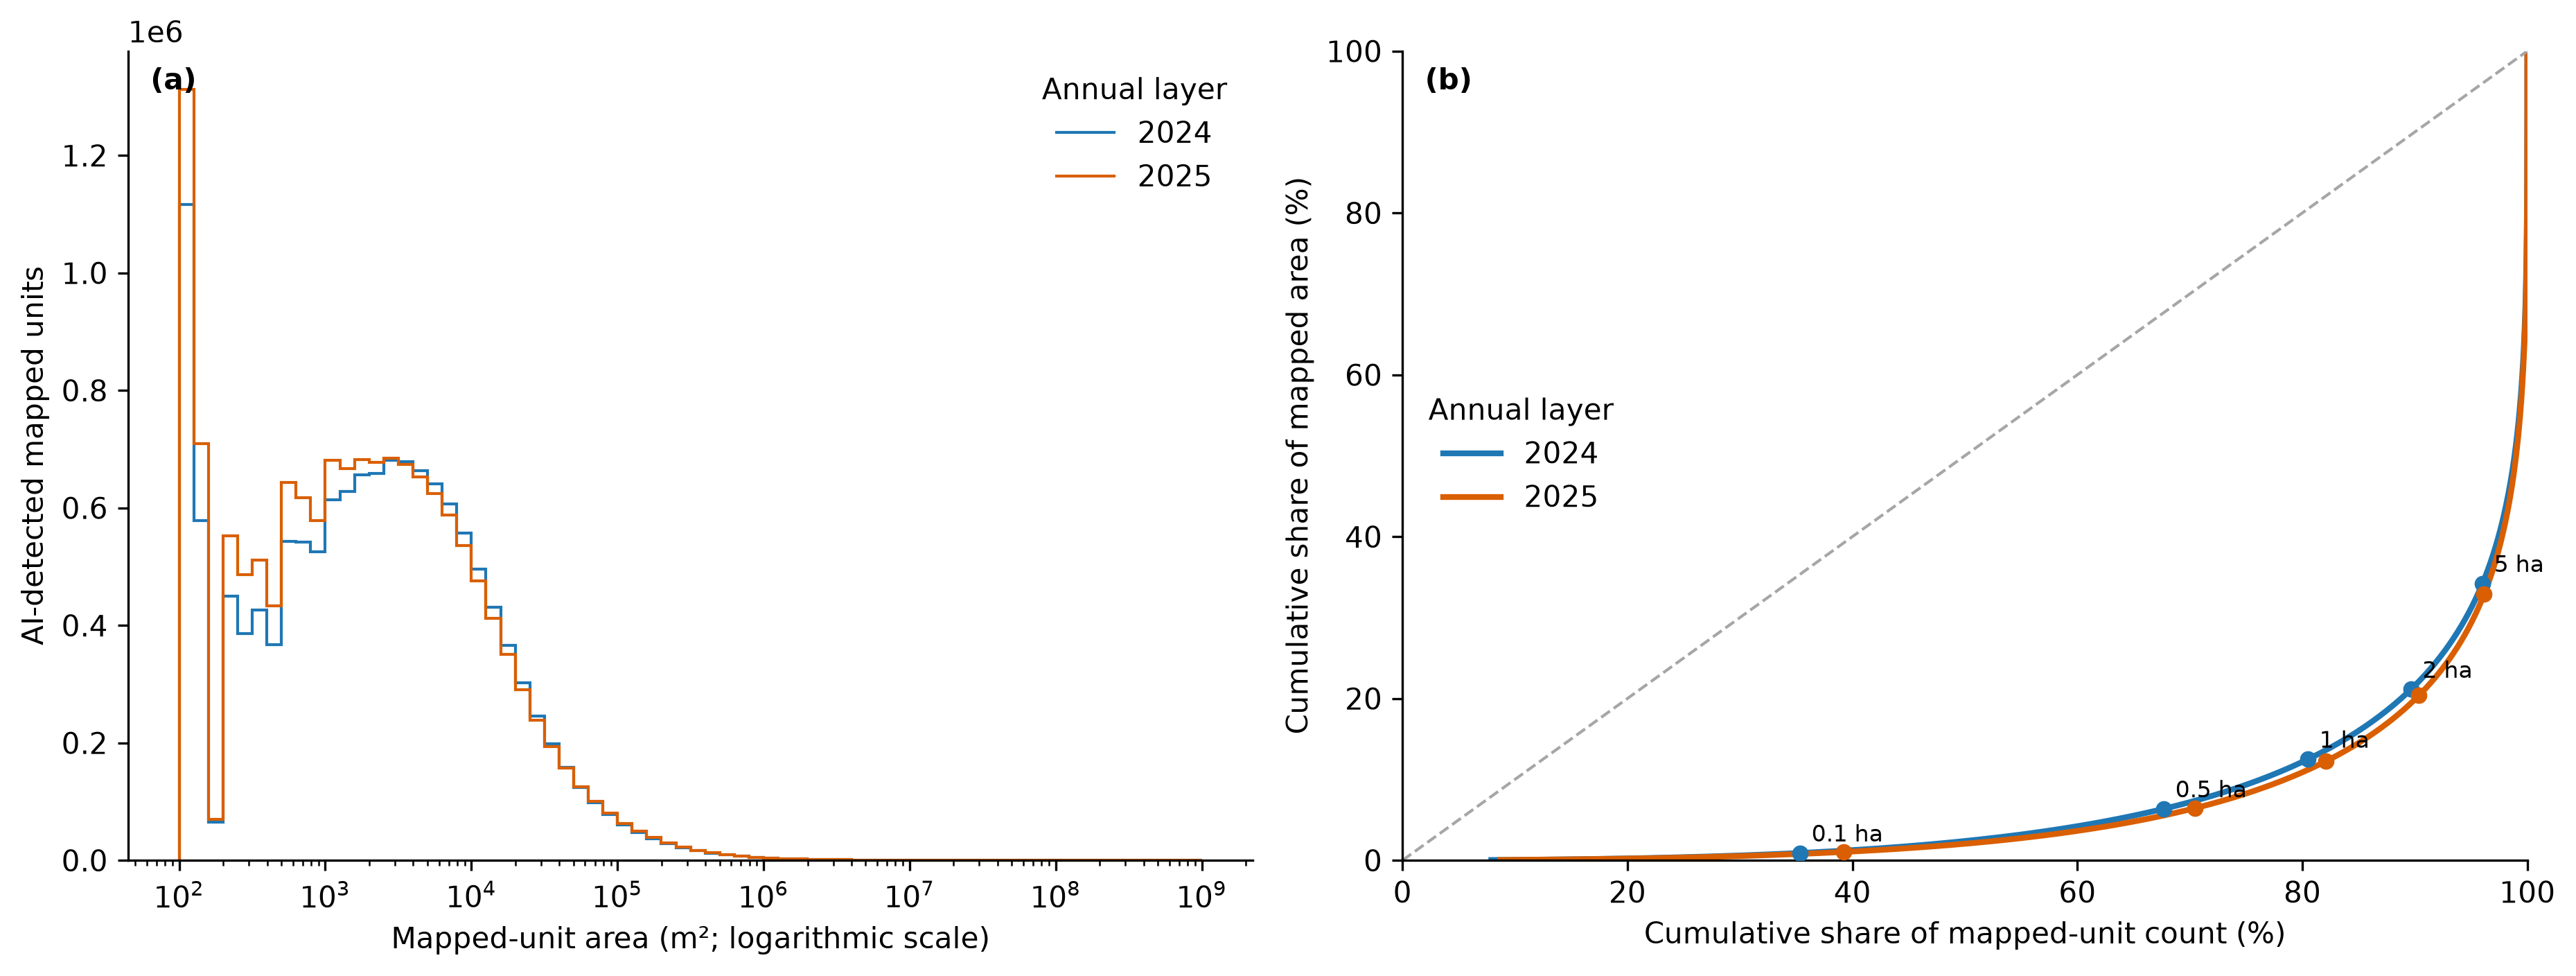
\includegraphics[width=\textwidth]{fig_1_national_area_distribution.png}
\caption{National mapped-unit area distributions and cumulative mapped-area concentration for the 2024 and 2025 product layers. The horizontal axis in panel (a) is logarithmic.}\label{fig:distribution}
\end{figure}

\subsection{Province and regional patterns and the effect of aggregation level}\label{subsec:province-results}

Figure~\ref{fig:spatial} visualises the 2024 province-level spatial distribution of median mapped-unit area, mapped-unit count per total province km$^{2}$ and mapped-unit count by 0.1$^{\circ}$ cell. Complete province and seven-region tables are supplied as machine-readable supplementary outputs. They show substantial within-country variation, including a cluster of extremely sparse coastal Black Sea provinces that is obscured by regional aggregation. Rize has no source record in either nominal layer.

This pattern must be interpreted through the target ontology established in Section~\ref{subsec:source}. FTW excludes perennial and tree-crop systems, pasture, permanent grassland, fallow and forestry. The present data contain neither an independent seasonal/annual-crop denominator nor reference boundaries with which to estimate omission. Terrain, imagery, compositing and model transfer may also matter, but their contributions are not identified. The coastal pattern is therefore an \emph{indeterminate target-class detection gap}, not evidence of a general agricultural ``coverage collapse'' or model failure. A user studying seasonal/annual crops in a sparse province must obtain target-matched reference evidence before drawing a substantive conclusion \citep{stehman_key_2019}.

Stage 5 exposes two further aggregation risks. National totals of the General Directorate of Mapping and equal-area Natural Earth province polygons are similar, yet their median absolute province discrepancy is 4.30\% and the maximum is 26.52\%. Individual mapped-unit-per-km$^{2}$ values and ranks therefore depend on the denominator. Regional averaging additionally hides the coastal sparsity. A defensible audit must report the finest supported unit, retain alternative denominators and match any rate denominator to the target ontology. Total province area is reproducible here, but it cannot turn mapped-unit counts into seasonal-crop detection rates.

\begin{figure}[t]
\centering
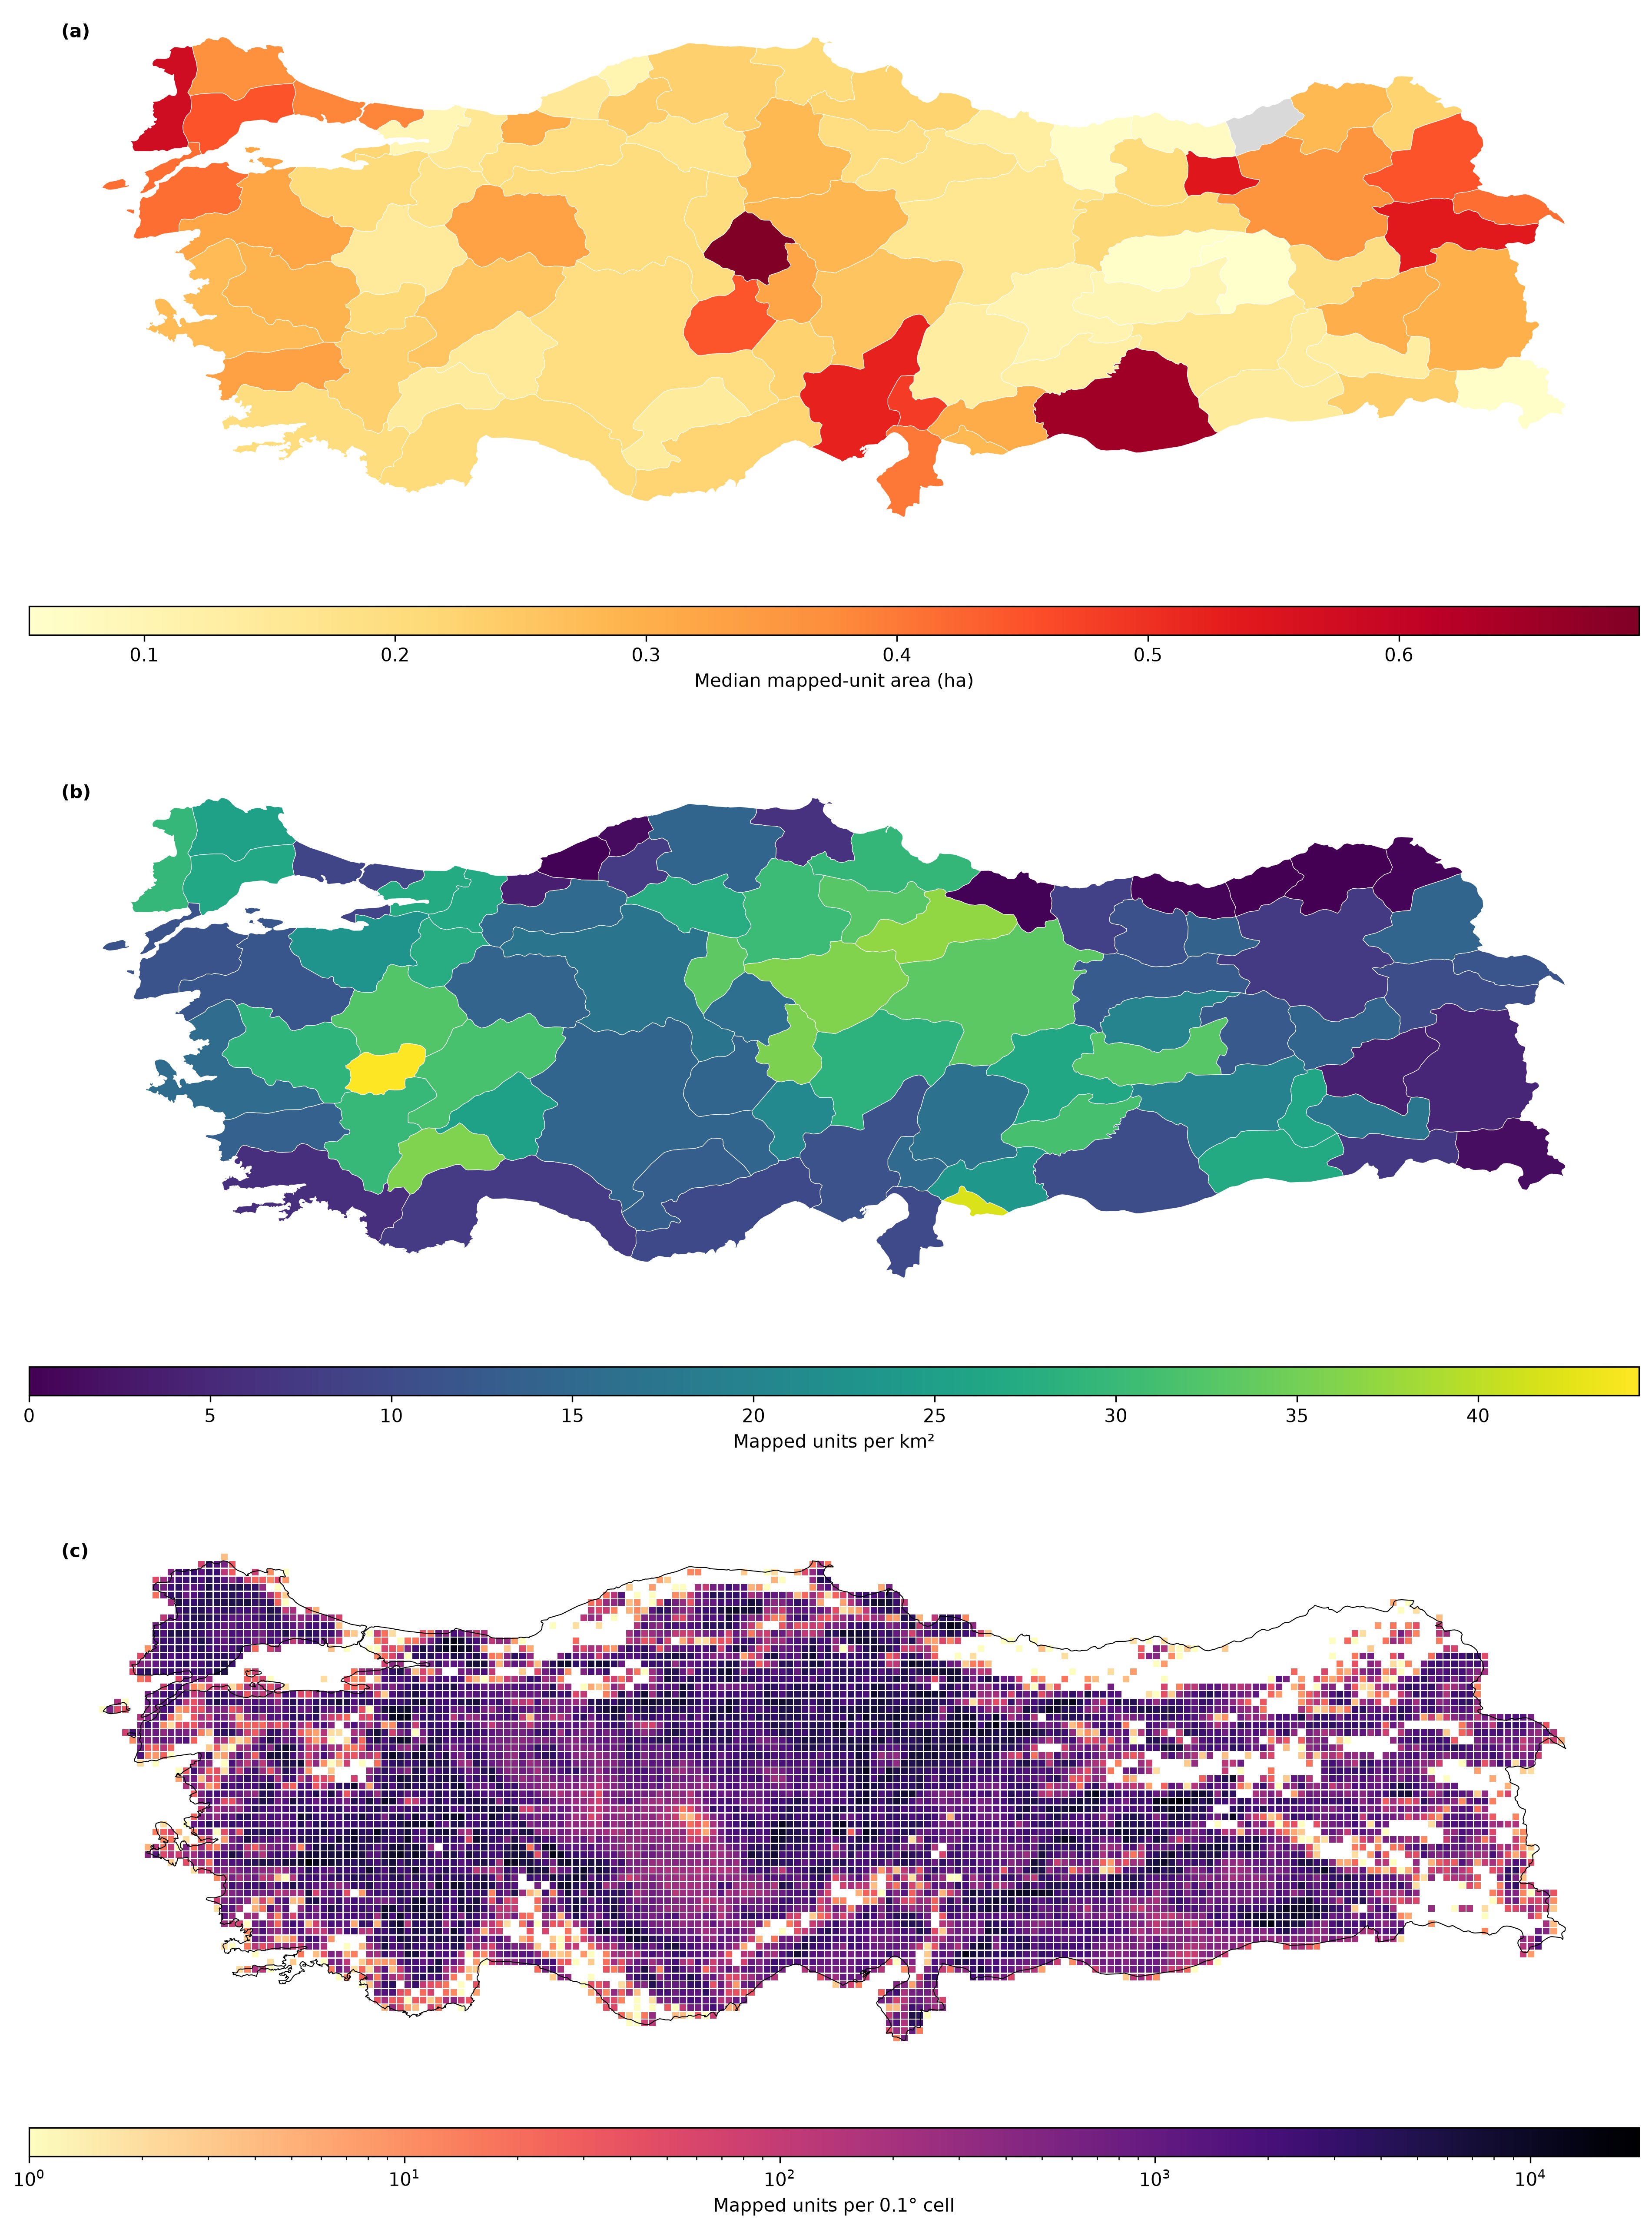
\includegraphics[width=\textwidth,height=0.78\textheight,keepaspectratio]{fig_2_spatial_patterns_2024.png}
\caption{Spatial distribution of the 2024 product layer. Panel (a) shows province median mapped-unit area, panel (b) mapped-unit count per total province km$^{2}$ using Turkish General Directorate of Mapping areas and panel (c) mapped-unit count by 0.1$^{\circ}$ cell assigned by bounding-box centre. Province statistics use HGM-derived analytical assignments, while public-domain Natural Earth outlines are used only for display. Grey denotes a province with no mapped unit and does not imply absence of FTW's target class.}\label{fig:spatial}
\end{figure}

\subsection{Confidence availability and sensitivity}\label{subsec:confidence-results}

Table~\ref{tab:confidence} reports confidence availability, non-null distributions and covered-subset threshold sensitivity for both nominal layers. Of the 2024 mapped units, 382,944 (2.708\%) have a non-null confidence value, and 407,060 (2.700\%) do so in 2025. The remaining 13,756,844 and 14,667,982 units have no sampled value because their points lie outside modelled-confidence coverage. Coverage share is therefore almost unchanged across layers and remains inadequate for national filtering. Among covered units, median confidence is 91.84 in 2024 and 90.42 in 2025 on the 0--100 vector scale. Their 10th-to-90th percentile ranges are 49.96--98.93 and 38.35--98.89. These are provider reliability values rather than external accuracy observations.

The documented 69 screen retains 307,668 covered units in 2024 and 304,156 in 2025. The 86 screen retains 246,750 and 241,501. Median mapped-unit area rises from 0.400 to 0.517 and 0.660 ha across the covered, 69 and 86 subsets in 2024, and from 0.358 to 0.532 and 0.691 ha in 2025. In both layers, screened subsets therefore differ systematically in size from the full covered subset. Applying either threshold to the national vector layer would remove approximately 97.3\% for missingness rather than observed low reliability. Stage 6 consequently passes for documented semantics, fails for national-filter availability and yields \emph{adopt with restrictions} only within the covered subset.

Figure~\ref{fig:confidence} provides the declared 2024 spatial diagnostic. Across 7,490 occupied 0.1$^{\circ}$ cells joined by 13,958 rook adjacencies, Moran's $I$ is 0.948 and 98.43\% of neighbouring pairs differ in null share by no more than ten percentage points. Of those cells, 7,183 are fully null, 237 mix null and non-null values and 70 are fully covered. The exported 2025 diagnostic contains 7,522 occupied cells, Moran's $I=0.969$ and 99.35\% of neighbour pairs within ten percentage points, with 7,204 fully null, 57 mixed and 261 fully covered cells. These large coefficients describe a concentrated pattern of missingness. They are not evidence of accuracy or a basis for causal interpretation. The available documentation does not explain the restricted footprint. Null meaning is taken from pinned provider metadata, not inferred from this pattern. Interpreting the uncovered 97.3\% as low confidence rather than unmeasured would reverse the documented meaning \citep{devillers_towards_2007,peng_call_2021}.

\begin{table}[t]
\caption{Confidence coverage, distribution and covered-subset sensitivity for both nominal product layers. Spatial diagnostics are finite-grid descriptors, and the figure maps 2024 for legibility.}\label{tab:confidence}
\centering
\footnotesize
\setlength{\tabcolsep}{3pt}
\begin{tabularx}{\textwidth}{@{}p{0.16\textwidth}YrrY@{}}
\toprule
Component & Measure & 2024 & 2025 & Interpretation \\
\midrule
Availability & Non-null count (share) & 382,944 (2.708\%) & 407,060 (2.700\%) & Available value \\
Availability & Null count (share) & 13,756,844 (97.292\%) & 14,667,982 (97.300\%) & Outside coverage; not low confidence \\
Distribution & 10th percentile & 49.96 & 38.35 & Covered subset only \\
Distribution & Median & 91.84 & 90.42 & Covered subset only \\
Distribution & 90th percentile & 98.93 & 98.89 & Covered subset only \\
Sensitivity & Covered: count; median area & 382,944; 0.400 ha & 407,060; 0.358 ha & No confidence threshold \\
Sensitivity & $\geq69$: count; median area & 307,668; 0.517 ha & 304,156; 0.532 ha & Covered subset only \\
Sensitivity & $\geq86$: count; median area & 246,750; 0.660 ha & 241,501; 0.691 ha & Covered subset only \\
Spatial diagnostic & Occupied cells; Moran's $I$ & 7,490; 0.948 & 7,522; 0.969 & Descriptive only \\
Spatial diagnostic & Neighbour pairs within 10 pp & 98.43\% & 99.35\% & Null-share difference \\
\botrule
\end{tabularx}
\end{table}

\begin{figure}[t]
\centering
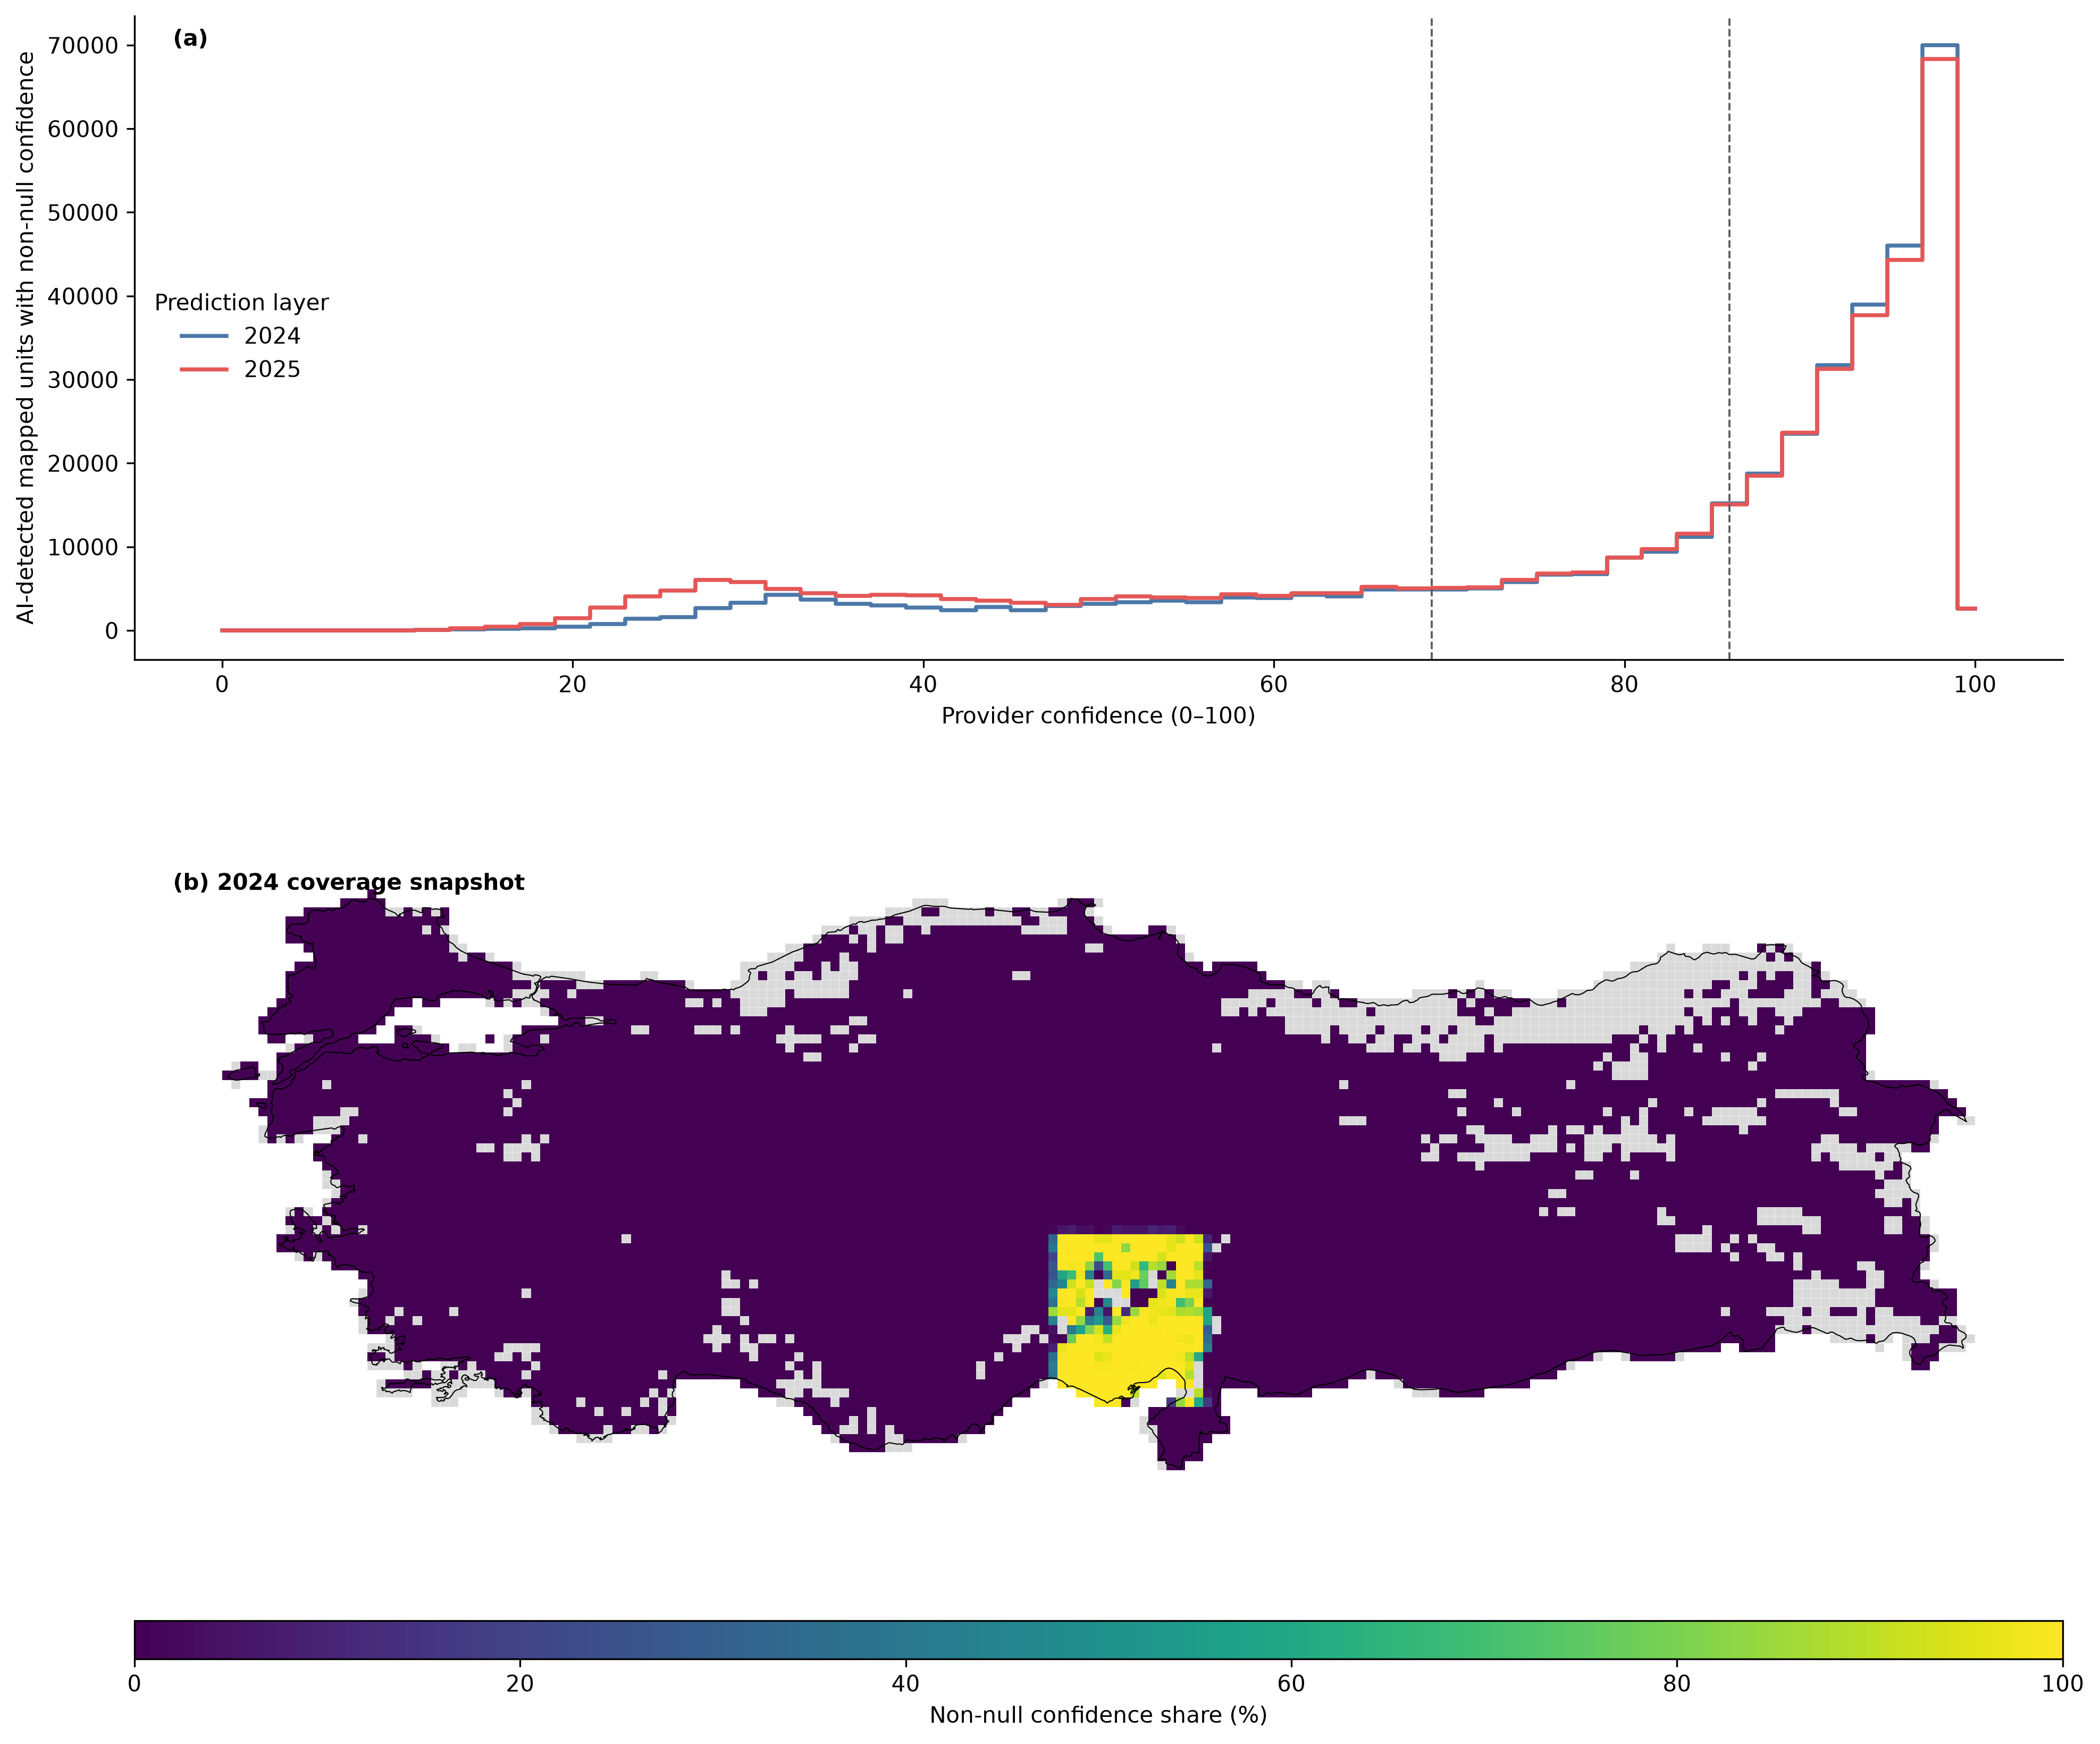
\includegraphics[width=\textwidth]{fig_3_confidence_2024_2025.png}
\caption{Confidence availability diagnostic. Panel (a) compares the distributions of non-null values in both nominal layers and marks the provider-documented threshold equivalents. Panel (b) maps the 2024 non-null share across occupied 0.1$^{\circ}$ cells assigned by mapped-unit bounding-box centre. Grey cells have no retained 2024 mapped unit under this procedure and do not imply absence of agriculture or of FTW's target class. Confidence coverage is not a polygon-accuracy surface.}\label{fig:confidence}
\end{figure}

\subsection{Cross-layer association, concordance and offsets}\label{subsec:agreement-results}

Figure~\ref{fig:agreement} visualises province aggregates for the nominal 2024 and 2025 layers against the one-to-one line. Table~\ref{tab:agreement} reports linear association, rank correspondence, concordance, province ratios and national output offsets. Mapped-unit count and summed polygon area show strong cross-layer correspondence. For count, Pearson's $r$ is 0.968, Spearman's $\rho$ is 0.939 and Lin's concordance correlation coefficient is 0.959 across 81 provinces. For summed polygon area, the corresponding values are 0.994, 0.985 and 0.994. Among 80 defined 2025-to-2024 province ratios, the count median is 0.989 with an interquartile range of 0.882--1.223. For summed area, the median is 1.031 with an interquartile range of 0.979--1.078. These coefficients are descriptive summaries of the enumerated provinces and can be elevated by persistent province size and target-class prevalence.

Median mapped-unit area has lower descriptive cross-layer correspondence. Across the 80 provinces with a defined median, Pearson's $r$ is 0.794, Spearman's $\rho$ is 0.804 and Lin's coefficient is 0.758. The province ratio median is 0.899 and its interquartile range is 0.785--1.039. Rize is excluded because both medians and every 2025-to-2024 ratio are undefined for its zero counts. No inference that one coefficient is statistically lower than another is made. The provinces are the finite reporting population rather than an independent random sample.

The national output offsets show why correlation alone is insufficient. Relative to the 2024 layer, the 2025 count is higher by 935,254 units (6.614\%), summed polygon area by 449,906 ha (2.134\%), and the median unit area is lower by 0.0384 ha (18.047\%). High province correspondence can therefore coexist with a systematic cross-layer offset. At the finer 0.1$^{\circ}$ grid, count Pearson, Spearman and Lin coefficients decline to 0.906, 0.905 and 0.900, and summed-area coefficients to 0.895, 0.930 and 0.894. Aggregation level therefore affects the apparent agreement. None of these offsets separates actual target-class or management change from imagery, mosaicking, masking, model behaviour or post-processing.

The distributional location of the offsets can be described without matching polygons. Of the net increase of 935,254 units, 914,595 (97.79\%) occurs below 0.1 ha, an 18.30\% rise within that band. The 0.1--0.5 ha band adds 139,839. Each intermediate band from 0.5 to 5 ha declines in count and summed area. The band at or above 5 ha rises by 15,380 units and 582,926 ha, so its summed-area gain exceeds the national net gain. The full decomposition is exported in the supplementary outputs.

The aggregate distribution is therefore not a uniform downward shift. It does not, however, identify splitting, merging, appearance, disappearance or real landscape change at polygon level, and local partitioning could coexist with changes in other bands. This result is retained only as a cross-layer diagnostic and is not evidence for a particular segmentation mechanism or for agricultural change. Stage 7 calculations are complete, but the evidence outcome is \emph{indeterminate} for change attribution and cannot support temporal monitoring without target-matched reference data.

\begin{table}[t]
\caption{Descriptive province-level association, concordance, ratios and signed national output offsets between the nominal 2024 and 2025 product layers.}\label{tab:agreement}
\centering
\footnotesize
\setlength{\tabcolsep}{3pt}
\begin{tabularx}{\textwidth}{@{}YrrrrrYY@{}}
\toprule
Outcome & $n$ & Pearson $r$ & Spearman $\rho$ & Lin CCC & Median ratio & Ratio IQR & National offset (\%) \\
\midrule
Mapped-unit count & 81 & 0.968 & 0.939 & 0.959 & 0.989 & 0.882--1.223 & $+935{,}254$ (6.614\%) \\
Summed polygon area & 81 & 0.994 & 0.985 & 0.994 & 1.031 & 0.979--1.078 & $+449{,}906$ ha (2.134\%) \\
Median mapped-unit area & 80 & 0.794 & 0.804 & 0.758 & 0.899 & 0.785--1.039 & \shortstack[r]{$-0.0384$ ha\\($-18.047$\%)} \\
\botrule
\end{tabularx}
\end{table}

\begin{figure}[t]
\centering
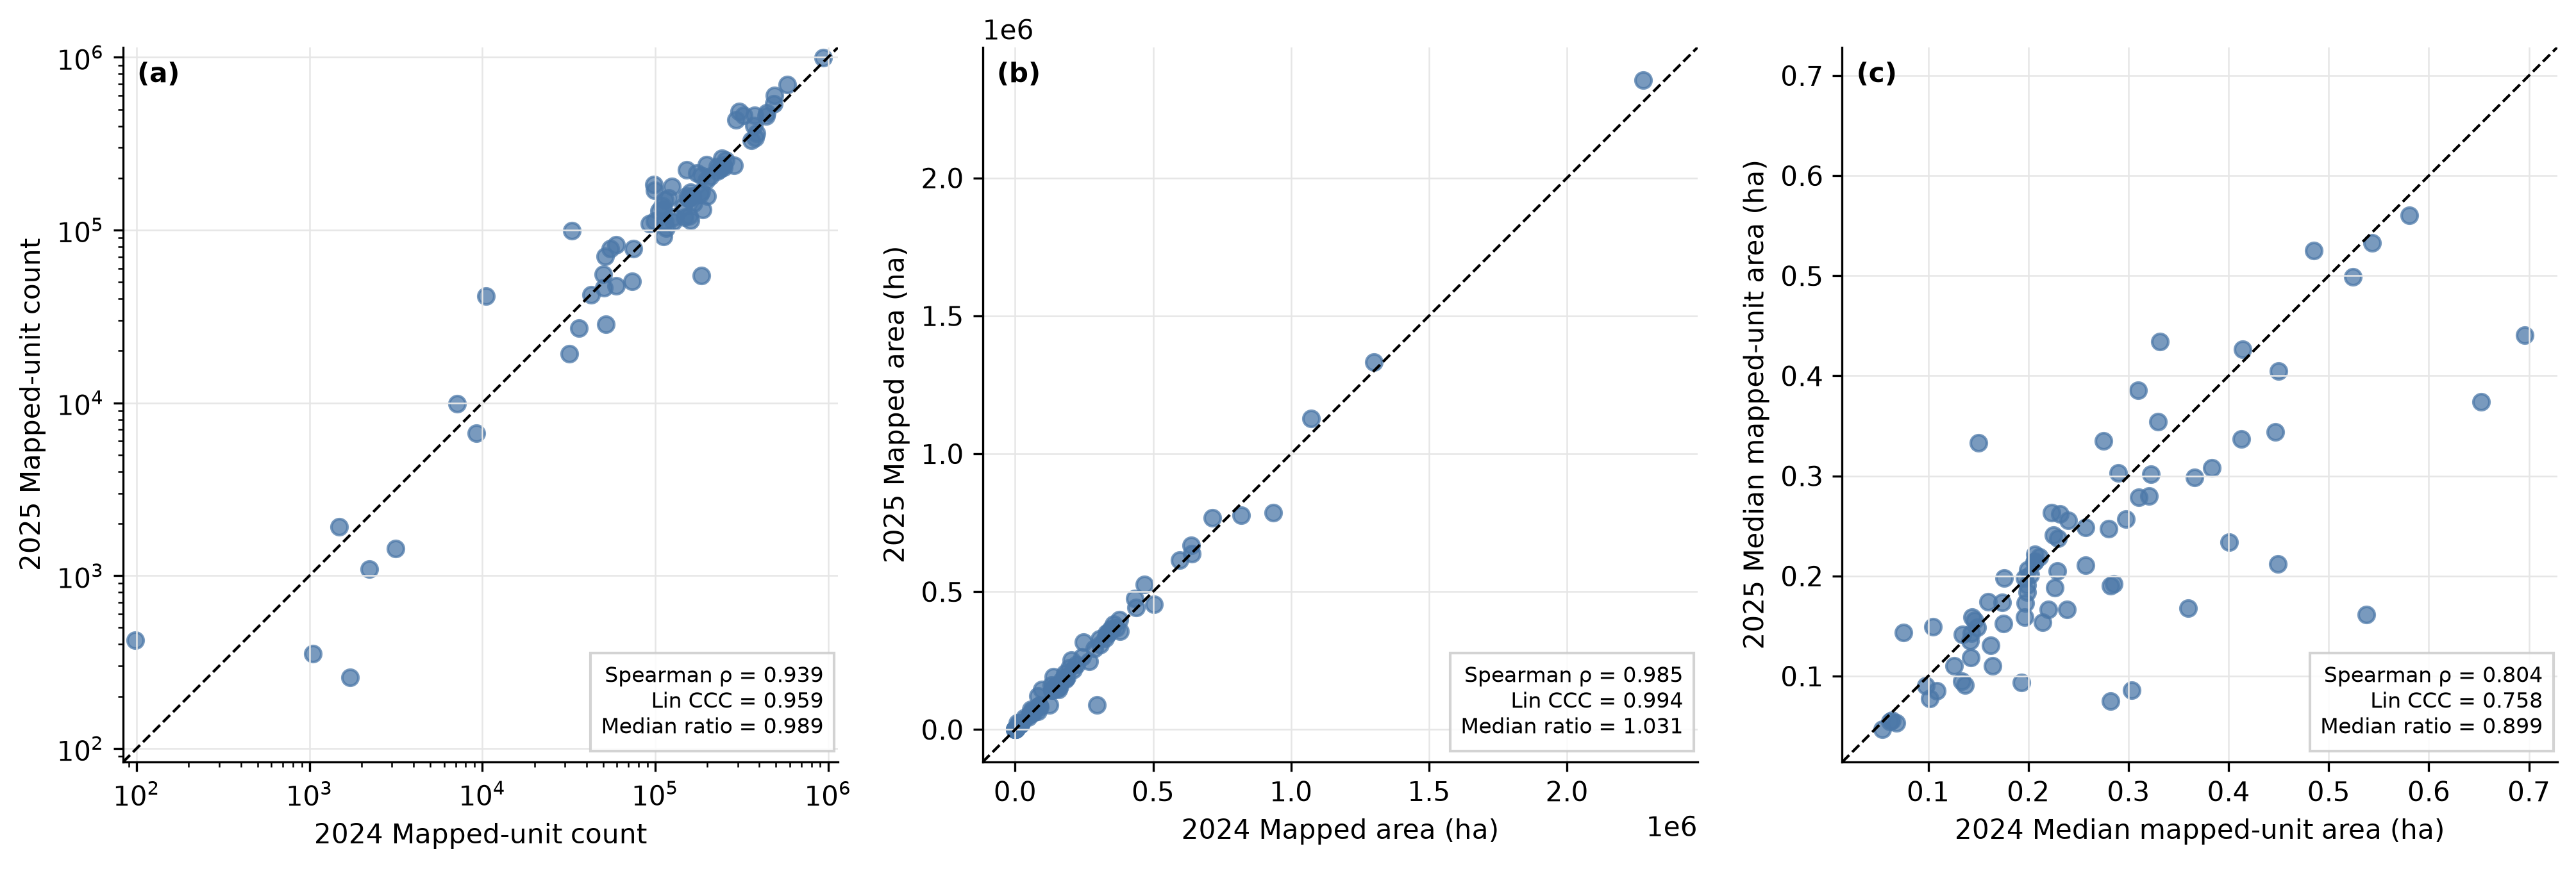
\includegraphics[width=\textwidth]{fig_4_cross_layer_consistency_2024_2025.png}
\caption{Descriptive province-level comparison of nominal 2024 and 2025 product layers for mapped-unit count, summed polygon area and median mapped-unit area. Dashed lines show one-to-one correspondence. Rank correlation, Lin concordance and median 2025-to-2024 ratios describe different properties and do not identify temporal change. Rize has zero count in both layers and undefined medians, so logarithmic panels omit its zero-valued point.}\label{fig:agreement}
\end{figure}

\subsection{Implications for agricultural and administrative use}\label{subsec:implications}

Table~\ref{tab:applications} applies the protocol's final decision rule rather than assigning the product one context-free quality score. The national partition and reproducible province summaries can support low-stakes exploration of FTW's seasonal/annual-crop target and prioritisation of locations for subsequent assessment. Any claim that depends on boundary accuracy, completeness, unique target-class area or change requires target-matched local reference data. Mapped size and shape may help prioritise locations for land-consolidation research \citep{alturk_shape_2024,yilmaz_evaluating_2025,yilgan_impacts_2026}, but cannot identify legal parcels or determine consolidation need.

These safeguards also define a data-governance boundary. FTW boundaries must not be used as evidence of ownership, cadastral extent, farm identity, ÇKS registration, subsidy entitlement or insurance liability without authoritative ground-based verification. Open access to a model output does not confer legal or administrative status. Downstream products should preserve product version, processing rules, known exclusions and the distinction between mapped units and people or registered entities. This is a provenance requirement in the sense of established provenance models \citep{missier_w3c_2013}. Reuse is safe only when the record of how a derived layer came about travels with it, which is also what the reusability principle of FAIR asks of published data \citep{wilkinson_fair_2016}. An open licence can permit redistribution subject to its terms, but it does not make an undocumented derivative interpretable.

\begin{table}[t]
\caption{Use-conditioned decisions returned by the protocol for the FTW Türkiye case. Decisions apply to the stated use, not to the product in the abstract.}\label{tab:applications}
\centering
\footnotesize
\begin{tabularx}{\textwidth}{@{}p{0.20\textwidth}p{0.17\textwidth}YY@{}}
\toprule
Stated use & Decision & Evidence permitted & Required safeguard \\
\midrule
Exploratory target-class inventory; sampling priorities & Adopt with restrictions & Compare mapped-unit distributions; target reference sampling & Preserve ontology, threshold scenarios, topology caveats and uncharacterised accuracy \\
Quantitative target-class extent or monitoring & External validation required & Design a target-matched probability sample & Estimate omission, commission, boundary and area error; report union area \\
Land-consolidation investigation & Adopt with restrictions & Flag locations for cadastral or field investigation & Do not treat mapped size or shape as legal geometry \\
Subsidy, insurance or eligibility & Reject for the declared use & Non-evidential quality-control overlay only & Use authoritative registries and verified parcels \\
Temporal or field-size change & External validation required & Describe cross-layer output under a fixed protocol & Require matched temporal reference data for change \\
Cadastral, ownership or legal boundary & Reject for the declared use & No evidential use & Require authoritative cadastral and administrative records \\
Confidence filtering & Adopt with restrictions for the covered subset; reject nationally & Filter documented non-null values only & Null is not low confidence; approximately 97.3\% is uncovered \\
\botrule
\end{tabularx}
\end{table}

\subsection{Limitations and provider-documentation ambiguity}\label{subsec:limitations}

The study does not estimate omission, commission or boundary accuracy, which requires an independent probability-based reference design \citep{olofsson_good_2014}. Nor does it observe the true prevalence of FTW's seasonal/annual-crop target in zero- or sparse-count areas. Reported counts and areas therefore characterise the pinned distributed output, not the complete number or extent of agricultural fields or even annual-crop fields in Türkiye. The confidence value is a provider model output at 500 m cell scale, not independent validation. The product is an alpha release, so results are tied to the accessed object checksum and must be rerun for later releases.

Minimum-area choice materially affects count, the small-unit tail and the absolute median even though summed polygon area and the conclusion that small units dominate count are comparatively stable. The provider-documented 400 m$^{2}$ scenario does not establish which post-processing rule generated each distributed polygon. Exact duplicate removal and validity checks also cannot establish semantic correctness. Extreme-size and topology diagnostics bound internal artefact risk but do not decide which geometry matches a target-class field on the ground. Shape index includes interior-ring boundary and therefore describes outline and inclusion structure together rather than exterior compactness alone.

The province rule is reproducible but depends on a point-on-surface decision and on polygons derived from the HGM display-purpose boundary product. Records straddling an international or province boundary can be assigned differently under another representation. The Natural Earth rerun therefore provides a sensitivity control rather than an alternative claim of legal authority. The complete crosswalk preserves provider code, both spatial assignments and every exclusion so that this dependence remains visible. HGM states that both its boundary product and its published area estimates are indicative rather than legally official, and its terms limit reuse to attributed, non-commercial purposes, so neither the source archive nor the derived boundary layer is redistributed here. The seven geographical regions are analytical conventions rather than administrative units.

The product documentation and the accompanying paper describe polygon production differently. The documentation and vector catalogue are pinned in the evidence package, but no provider clarification is claimed. The ambiguity cannot explain the observed cross-layer offsets. Actual target-class change, imagery, compositing, masks, model behaviour, post-processing and minimum-mapping behaviour remain inseparable without additional evidence.

Two comparisons a reader might expect are deliberately not made. Comparing FTW medians with official parcel or holding statistics would combine different populations, units and summaries, inviting an undefined error or fragmentation interpretation. Comparing summed polygon area with national agricultural area would additionally violate the FTW target ontology and ignore overlaps. The eighth General Agricultural Census began in July 2025. The Turkish Statistical Institute stated that first results were planned for the second half of 2026, and none were listed as published by the 31 July 2026 analysis date \citep{turkish_statistical_institute_general_census_2026}. Even a current all-agriculture total would not be a target-matched accuracy reference.

The protocol was developed and exercised by one author on a single product in one country. No independent analyst, user institution, second product type or formal consensus exercise has yet tested stage interpretation, inter-rater agreement, execution time or completeness. The method should therefore be treated as a transparent, falsifiable proposal rather than a validated standard. This limitation narrows the generalisability claim but not the reproducibility of the worked evidence. Neither layer is treated as direct observation of agricultural change, and no result supports cadastral, holding, farm, ownership or ÇKS inference.

\section{Conclusions}\label{sec:conclusions}

This study contributes a use-conditioned, reproducible due-diligence protocol for evaluating open AI-derived Earth-observation products before adoption. It complements ISO 19157-1 and ISO 19131, FAIR, PROV and producer documentation by converting available quality information into auditable evidence states and one of four use-specific actions. Administrative scope, target ontology, geometry and topology, metric quality, threshold sensitivity, attribute semantics, denominators, cross-layer consistency and reproduction are made explicit and testable.

Applied to FTW over Türkiye, stage 1 establishes two facts that condition every other result: no country-specific reference evaluation is reported for Türkiye, and the product targets seasonal or annual crops rather than all agriculture. The as-distributed analytical populations contain 14.14 and 15.08 million mapped units with 21.08 and 21.53 million ha of summed polygon area. Exact tiled unions show negligible repeated footprint, but units at or above 100 ha contribute 28--29\% of those sums. The documented 400 m$^{2}$ scenario removes 21--24\% of units and raises medians by 68--85\%, while changing summed area by less than 0.33\%. Confidence is absent for approximately 97.3\% in both layers and cannot support national filtering. Province aggregates correspond strongly across layers, but systematic offsets remain and their causes are not identifiable from the product alone.

The resulting decision is conditional rather than promotional. FTW receives \emph{adopt with restrictions} for exploratory target-class characterisation and reference-sample prioritisation, \emph{external validation required} for quantitative extent, accuracy or change inference, and \emph{reject for the declared use} for cadastral, registry, eligibility, ownership or other rights-affecting decisions. Broader claims for the protocol itself require independent users and further product classes.

\backmatter
\hypersetup{bookmarksdepth=4}
\bmhead{Supplementary information}

Online Resource 1 contains the protocol JSON Schema, the completed decision record, the executable workflow, the environment specification, the machine-readable result tables and the instructions needed to rebuild the administrative layer locally. The FTW object, the HGM archive and the boundary layer derived from it are not redistributed. Their retrieval locations, checksums and derivation steps are supplied so that users who accept the source terms can reproduce the analysis.

\section*{Statements and Declarations}

\bmhead{Funding}
This research received no external funding.

\bmhead{Competing interests}
The author declares no competing interests.

\bmhead{Ethics approval and consent to participate}
Not applicable.

\bmhead{Consent for publication}
Not applicable.

\bmhead{Data availability}
The Fields of The World global prediction dataset is publicly available through Source Cooperative at \url{https://source.coop/ftw/global-data} under CC BY 4.0. This study uses the Türkiye alpha partition, accessed on 18 July 2026. The HGM boundary product is available from \url{https://www.harita.gov.tr/urun/turkiye-mulki-idare-sinirlari/232} and was accessed on 31 July 2026. HGM describes the boundary data as display-purpose and non-official, requires attribution and limits reuse to non-commercial purposes, so neither the HGM archive nor the boundary layer derived from it is redistributed. Version identifiers and checksums for every input are recorded in the reproducibility package at \url{https://github.com/yunusserhat/ftw-turkiye-reproducibility}.

\bmhead{Materials availability}
Not applicable.

\bmhead{Code availability}
Analysis code and generated outputs are maintained at \url{https://github.com/yunusserhat/ftw-turkiye-reproducibility}. Author-written code is released under the GNU General Public License v3.0, and author-generated documentation, tables and figures under CC BY 4.0. Third-party data retain the licences of their original sources. The workflow verifies source checksums, applies the documented audit rules and regenerates the machine-readable tables and figures. Numerical checks use exact integer equality or declared floating-point tolerances.

\bmhead{Author contributions}
Y.S.B.: conceptualisation, data curation, formal analysis, methodology, software, visualisation, writing---original draft, and writing---review and editing.

\bibliography{sn-bibliography}

\end{document}
